

\subsection{Applying Kernel PCA}

\begin{frame}{\subsecname}

\question{How do I interpret the role of PCs?}

\begin{center}
	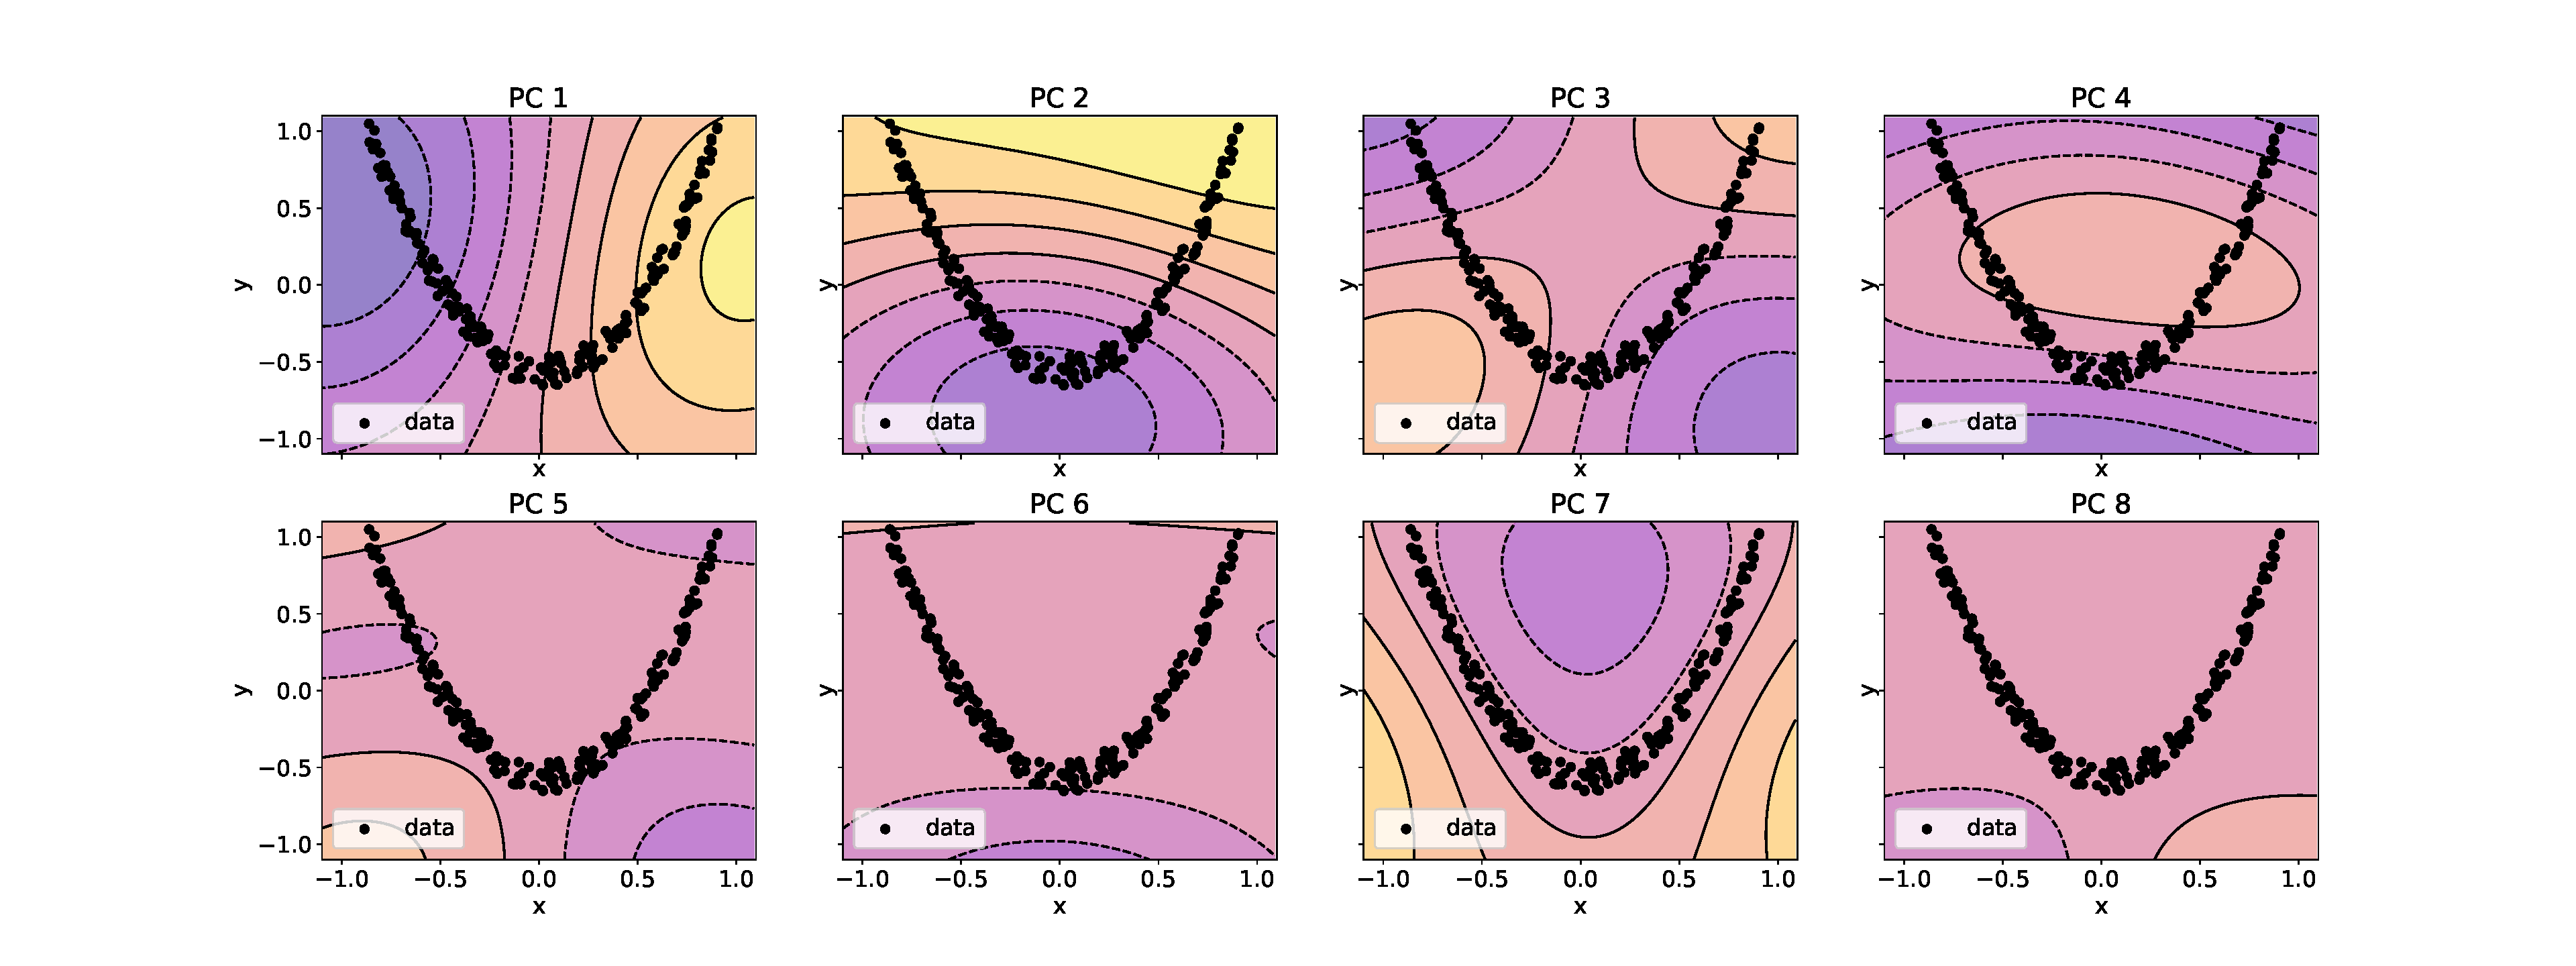
\includegraphics[height=5cm]{img/contourplot_kpca_rbf}
	\captionof{figure}{Projections onto individual PCs}
\end{center}

\end{frame}

\subsection{A note on implementation}

\begin{frame}{\subsecname}

\question{Should you solve the transformed eigenvalue problem using \emph{eigenvalue decomposition} or \emph{SVD}?}

\slidesonly{
\begin{equation}
%\label{eq:eigsimple1}
	\vec{K} \, \vec{a} = p \lambda \vec{a}
\end{equation}
}

\pause

- \emph{eigenvalue decomposition} is the only option for Kernel PCA. \emph{SVD} is simply not applicable since we don't have access to $\vec \phi_{((\vec x))}$

\begin{equation}
 %\label{eq:cov}
\vec C_{\phi} = \frac{1}{p} \sum_{\alpha=1}^{p} \vec{\phi}_{(\vec{x}^{(\alpha)})} \vec{\phi}^{\top}_{(\vec{x}^{(\alpha)})}
\end{equation}

\end{frame}

\begin{frame}{\subsecname}

\question{Which property of $\widetilde {\vec{K}}$ can we exploit to speed up computation?}

\pause

The kernel function is symmetric. $k(\vec x^{(\alpha)}, \vec x^{(\beta)}) = k(\vec x^{(\beta)}, \vec x^{(\alpha)})$. One can exploit this by reducing how many times the kernel function is actually applied while traversing the training samples when computing $\widetilde {\vec{K}}$.

\end{frame}
